\chapter{Slowly decaying eigenmodes\label{chap:currents}}
\thispagestyle{chapterBeginStyle}

In the previous chapter, we have numerically shown the existence of optimal anisotropy
\(\Delta_{O} = \exp(- \alpha + 2)\), which ensures slow relaxation of the spin current
 \(j^{\sigma}\)~\eqref{eq:spin_current} and consequently quasiballistic spin transport.
 Here, we will demonstrate that this feature is not unique to the spin current, but
 exhibited also by a class of other, \textit{local} operators. To this end, we will
 employ an algorithm devised by \textcite{Mierzejewski2015a}, originally designed to
 identify local integrals of motion in integrable tight-binding models. As the model
 we are considering in this work is not integrable, we are not expecting to find
 strictly conserved quantities, but only so-called \textbf{local slowly relaxing
 operators (LSROs)}. We will interpret the discovered observables in terms of
 fermionic currents, describing particle hopping with various ranges.
 Moreover, we will also show how to improve the numerical efficiency of
 the algorithm, by utilizing symmetry subspaces and the Dynamical Quantum Typicality
 approach to correlation functions\footnote{And why it, unfortunately, fails in this case.}
(cf. section~\ref{sec:DQT}).


\section{Detecting local slowly relaxing operators \label{sec:slowly_relaxing_operators}}
\subsection{Theoretical description}
Let us start by introducing in detail the original algorithm for detecting local integrals
of motion (LIOMs), following the original article by~\autocite{Mierzejewski2015a}.
In principle, finding a \textbf{complete set of LIOMs} is a conceptually
nontrivial task, however, this procedure reduces it to a simple application of linear algebra~\autocite{Mierzejewski2015a}.
In this section, unless stated otherwise, by \(H\) we will denote an arbitrary
tight-binding Hamiltonian with periodic boundary conditions
on \(L\) sites, having eigenstates \(H \ket{n} = \epsilon_{n} \ket{n}\). Moreover,
for any operator \(A\) we define \(A_{mn} \equiv \matrixel{m}{A}{n}\).

In order to employ techniques from linear algebra, we need to have a linear space of some kind.
This role is played by the space of \textit{local, traceless, and translationally invariant} operators,
supported on up to \(M\) sites and acting on vectors from a Hilbert space \(\mathcal{H}\) of 
dimension \(\mathcal{D}\). We will denote this space by \(\mathcal{V}_{M}\). Its building blocks are the
spaces \(\mathcal{V}^m\), of operators supported on exactly \(m\) sites, i.e. of the form
\begin{center}
    \hspace*{-0.5cm}
    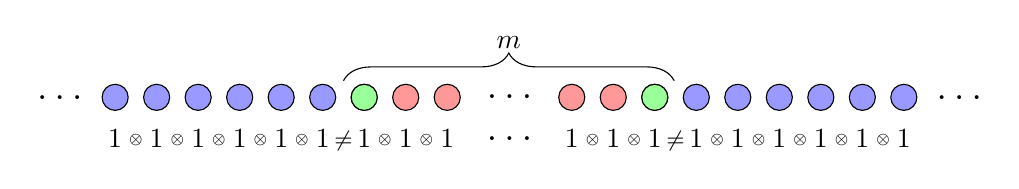
\begin{tikzpicture}[node distance = 15pt, auto]
        \tikzstyle{line} = [draw, -latex',thick]
        \tikzstyle{site1}=[circle, draw, fill=blue!40]
        \tikzstyle{site2}=[circle, draw, fill=red!40]
        \tikzstyle{site3}=[circle, draw, fill=green!40]
        % Place nodes
    
        \node [site1] (site-1) at (-8, 0) {};
        \foreach \x / \name in {1/2,2/3,3/4,4/5,5/6}
        \node [site1, right of=site-\x] (site-\name) {};
    
        \node [site2, right of =site-6] (site-7){};
        \foreach \x / \name in {7/8,8/9}
        \node [site2, right of=site-\x] (site-\name) {};
    
        \node [site2, right of=site-9, node distance=45pt] (site-10){};
        \foreach \x / \name in {10/11,11/12}
        \node [site2, right of=site-\x] (site-\name) {};
    
        \node[site1, right of=site-12] (site-13){};
        \foreach \x / \name in {13/14,14/15,15/16,16/17,17/18}
        \node [site1, right of=site-\x] (site-\name) {};
    
        \node [left of=site-1, node distance=20pt] {\Large $ \ldots $};
        \node [right of=site-18, node distance=20pt] {\Large $ \ldots $};
    
        \node [site3, right of=site-6] (site-X) {};
        \node [site3, right of=site-11] (site-X) {};
    
        \foreach \x in {1,...,18}
        \node [black, below of=site-\x](op-\x) {\(\mathbb{1}\)};
    
        \foreach \x / \y in {1/2,2/3,3/4,4/5,5/6,7/8,8/9,10/11,11/12,13/14,14/15,15/16,16/17,17/18}
        \path[draw=none] (op-\x) -- (op-\y) node [black,midway,yshift=-6pt] {\tiny$\otimes$};
    
        \path[draw=none] (op-6) -- (op-7) node [black,midway,yshift=-8pt] {\footnotesize$\neq$};
        \path[draw=none] (op-12) -- (op-13) node [black,midway,yshift=-8pt] {\footnotesize$\neq$};
        % \foreach \x in {-1.5,-1.0,-0.5,0.5,1.0,1.5}
        % \node [site2] (site-\x) at (\x, 0) {};
    
        \draw [decorate,decoration={brace,amplitude=10pt},yshift=6pt]
        (-5.1,0) -- (-0.9,0) node [black,midway,yshift=8pt] {$m$};
    
        \path [draw=none] (site-9) -- (site-10) node [black,midway,yshift=-4pt] {\Large$\ldots$};
        \path [draw=none] (op-9) -- (op-10) node [black,midway,yshift=-4pt] {\Large$\ldots$};
      \end{tikzpicture}    
\end{center}    
where blue circles correspond to single-site identity operators, green circles to an arbitrary
single-site operator except for the identity and red circles to an arbitrary single-site operator.
If we were to allow identity operators on green sites, we would have obtained a \((m-1)\)-local operator.
It is easy to see that an arbitrary linear combination of operators from \(\mathcal{V}^m\) is again
an element of \(\mathcal{V}^m\), hence \(\mathcal{V}^m\) is a linear space. Therefore,
the full space
\begin{equation}
    \mathcal{V}_{M} = \bigoplus_{m=1}^{M} \mathcal{V}^m
\end{equation}
is also a linear space. We will always assume that \(0\leq M \leq L/2\).

Using the infinite temperature correlation function (cf. Eq.~\eqref{eq:corr_fun}) we can endow this space with an inner product
\begin{equation}
    \mathcal{V}_M \cross \mathcal{V}_M \ni (A, B) \mapsto \hs{A}{B}
    \equiv \frac{1}{\mathcal{D}}\Tr\left(AB\right) = \frac{1}{D}\sum_{n,m = 1}^{D} A_{nm} B_{nm}^{\ast} \in \CC
    \label{eq:hs_prod}
\end{equation}
called the \textbf{Hilbert-Schmidt inner product} and
inducing the \textbf{Hilbert-Schmidt norm} \(\norm{A} = \sqrt{\hs{A}{A}}\).
Because we only consider finite systems in this thesis, we do not need to worry about
situations where the trace is not well defined. The pair \( (\mathcal{V}_M, \hs{\cdot}{\cdot}) \)
is then a finite-dimensional Hilbert space.
We are now able to state more precisely what we mean by a complete set of LIOMs.
It is a set of local operators \(\{Q_{\alpha} : \comm{Q_{\alpha}}{H} = 0\}\), such that
for any observable \(A\) we have
\begin{equation}
    \lim_{t\to\infty} \hs{A(t)}{A} = \sum_{\alpha} \frac{\hs{Q_{\alpha}}{A}^2}{\hs{Q_{\alpha}}{Q_{\alpha}}}
\end{equation}
i.e. the completeness is understood as the saturation of the Mazur bound~\autocite{Mazur1969}.

The mathematical stage is now set, so let us proceed further toward the algorithm. 
As \(\mathcal{V}_M\) is a linear space, it possesses a basis \(\{O_{s}\}\),
which with the help of the inner product can be made into an orthonormal basis \(\hs{O_s}{O_{t}} = \delta_{st}\).
We can also think of this space as an orthogonal subspace of the space \(\mathcal{V}\) of all possible operators
acting on \(\mathcal{H}\), in the sense that
\begin{equation}
    \big(\forall A \in \mathcal{V} \big) \big( A = A^M + A^{\perp} = \sum_s \hs{O_s}{A} O_s + A^{\perp}\big) ,
    \text{ such that } \big(\forall s\big) \big( ({O_s}|{A^{\perp}}) = 0\big)
    \label{eq:decomposition}
  \end{equation}
We will describe an example of such a basis in the next section, but for now, it is enough that it exists.

Next, we would like to determine the conserved part of all the basis operators \(O_s\). We do this
by considering the infinite time average 
\begin{align}
    \bar{O}_s = \lim_{\tau\to\infty}\frac{1}{\tau} \int_0^{\tau} \mathrm{d}t\, O_s(t) &= 
     \lim_{\tau\to\infty}\frac{1}{\tau} \int_0^{\tau} \mathrm{d}t\, \mathrm{e}^{i H t}O_s \mathrm{e}^{-i H t} \nonumber\\
     &= \sum_{m,n} (O_s)_{mn}\ketbra{m}{n} \lim_{\tau\to\infty} \frac{1}{\tau} \int_0^{\tau} \mathrm{d}t \, \mathrm{e}^{i(E_m-E_n)t} \nonumber\\
    &= \sum_{\substack{n,m \\ E_n = E_m}} (O_s)_{mn}\ketbra{m}{n}
    \label{eq:time_avg}
\end{align}
This time-averaging amounts to a cut-off, removing all matrix elements between non-degenerate eigenstates
of the Hamiltonian. A crucial property of this operation is that it is an orthogonal projection
in the space of operators, i.e. \(\hs{\bar{O}_s}{\bar{O}_t} = \hs{\bar{O}_s}{O_t}\). This will
in the end will allow us to distinguish between different types of conserved quantities.
However, our ultimate goal concerns LSROs in a system that is not integrable, which dictates the
need for performing also a finite-time averaging. Unfortunately, a simple omission of the limit
in Eq.~\eqref{eq:time_avg} destroys the projective character of this operation. To remedy this,
we introduce a parameter \(\tau\) and define effective time averaging~\autocite{Mierzejewski2015}
as
\begin{equation}
    \bar{O}_s^{\tau} = \int_{-\infty}^{\infty} \mathrm{d}t\, O_s(t) \frac{\sin(t/\tau)}{\pi t}
\end{equation}
By considering the Fourier transform of the \(\sin(x)/x\) function, it can be shown that
this expression is equivalent to (\textcolor{red}{Appendix C if time permits})
\begin{equation}
    \bar{O}_s^{\tau} = \sum_{n,m} \underbrace{\theta\left(\frac{1}{\tau} - |E_n - E_m|\right)}_{\theta_{mn}^{\tau}} (O_s)_{mn} \ketbra{m}{n}
\label{eq:finite_time_avg}
\end{equation}
and because for Heaviside theta function we have \(\theta(x)^2 = \theta(x)\), the projective character is restored. Notice the similarity
of this expression to the integrated conductivity~\eqref{eq:integrated_conductivity}. Indeed, the 
parameter \(1/\tau\) can be interpreted as \(\Omega\), giving the frequency cut-off for the matrix elements.
Properties the \(\theta\)-function ensure that the \(\tau\to\infty\) limit of Eq.~\eqref{eq:finite_time_avg}
agrees with Eq.~\eqref{eq:time_avg}. Let us now calculate the commutator of \(O_s^{\tau}\) with the Hamiltonian
\begin{align}
    \comm{H}{\bar{O}_s^{\tau}} & = \sum_n \sum_{k,p} \epsilon_n \theta_{kp}^{\tau} (\bar{O}_s)_{kp} \comm{ \ketbra{n}{n}}{ \ketbra{k}{p}} \nonumber         \\
                             & = \sum_{k,p} \left(\epsilon_k-\epsilon_p\right) \theta_{kp}^{\tau} (\bar{O}_s)_{kp} \ketbra{k}{p} \xrightarrow{\tau \to \infty} 0 
        \label{eq:time_averaged_commutator}
\end{align}
We see that the operator obtained from infinite-time averaging is an integral of motion. Unfortunately,
this procedure modifies the support of the operator and in general \(\bar{O}_s \not\in \mathcal{V}_M\).

Having calculated the time-averaged basis \( \{\bar{O}_s^{\tau}\} \), we would like to perform in a 
systematic way the decomposition~\ref{eq:decomposition}. We need the overlaps between the basis operators
before and after the time-averaging. Because of the projective character of the time-averaging, they are
given by the pairwise inner products of the time-averaged operators, which we collect into a matrix
\(K^{\tau}\), with elements
\begin{equation}
    K^{\tau}_{st} = \hs{\bar{O}_s^{\tau}}{\bar{O}_t^{\tau}} = \sum_{n,m} \theta_{mn}^{\tau} (O_s)_{nm} (O_t)_{nm}^{\ast}
\end{equation}
This matrix is Hermitian by design, and in the case of systems with time-reversal symmetry, it is also real,
thus symmetric. By the spectral theorem, there exists a unitary matrix \(U\) that diagonalizes it
via a similarity transformation with the following properties
\begin{align}
    &\sum_{s, t} U_{n s} K_{s t}^{\tau} U_{m t}^{\ast}=\delta_{nm} \lambda_{n} \in
     \RR,\;\;\; \lambda_n \text{ --- eigenvalue of }K^{\tau} \label{eq:property diag} \\
    &UU^{\dag} = U^{\dag}U = \mathbb{1} \implies \sum_{s} U_{ns}U_{ms}^{\ast} =
     \delta_{mn} \label{eq:propery_ortho}\\
    & U K^{\tau} = D U \implies \sum_s U_{ns} K_{st}^{\tau} = \sum_s  \delta_{ns} \lambda_s U_{st} = \lambda_n U_{nt}\label{eq:property}
  \end{align} 
Using the columns of \(U\), which are just the eigenvectors of \(K^{\tau}\), we can construct a new set of operators
\begin{equation}
    Q_{n} = \sum_{s} U_{n s} \bar{O}_s^{\tau}
    \label{eq:liom}
\end{equation}
Let us note a few properties of the newly defined quantities. First, they are orthogonal
\begin{align}
    \hs{Q_n}{Q_m} &= \sum_{s,t} U_{ns} {\hs{\bar{O_s}^{\tau}}{\bar{O_t}^{\tau}}} U_{mt}^{\ast} 
    = \sum_{t} \left(\sum_{s}U_{ns} K_{st}^{\tau}\right)  U_{mt}^{\ast}\nonumber \\ 
    &= \lambda_n \sum_t U_{nt} U_{mt}^{\ast} = \lambda_n \delta_{mn}
  \end{align}
where the last two equalities follow from~\eqref{eq:property} and~\eqref{eq:propery_ortho} respectively.
From the fact that \(\hs{Q_n}{Q_n} = \lambda_n\) and that \(\hs{\cdot}{\cdot}\) is an inner product,
we immediately deduce that \(K^{\tau}\) is positive semidefinite.
We are now ready to consider the desired decomposition into the part that is supported on at most \(M\) sites and the remaining, nonlocal part
\begin{align}
    Q_n &=  \sum_s \hs{O_s}{Q_n}O_s + Q_n^{\perp} = \sum_{s,t} U_{n t}\hs{O_{s}}{\bar{O}_{t}^{\tau}}
    O_{s}+Q_{n}^{\perp} \nonumber \\
    &= \sum_{s,t} U_{n t}\hs{\bar{O}_{s}^{\tau}}{\bar{O}_{t}^{\tau}} O_{s}+Q_{n}^{\perp}
    = \sum_{s,t} U_{n t}K_{ts} O_{s}+Q_{n}^{\perp} \nonumber \\
    &= \sum_s  \left( \sum_t U_{n t}K_{ts}^{\tau}\right) O_{s}+Q_{n}^{\perp} = \sum_{s} 
    \lambda_{n} U_{n s} O_{s}+Q_{n}^{\perp} = Q_{n}^{M}+Q_{n}^{\perp}
    \label{eq:decomposition2}
  \end{align}
  Everything we did so far holds for an
arbitrary value of \(\tau\). However, let us for a moment restrict it to \(\tau\to \infty\).
This guarantees that the operators \(Q_n\) are integrals of motion.
  We have one step left to complete the algorithm and obtain a classification scheme for the
  integrals of motion. We need to determine how much of the operator \(Q_n\) is contained in the
  \(M\)-local part \(Q_n^M\). In other words, we want to calculate \(\norm*{Q_n^{\perp}}\).
  Consider the following calculation
  \begin{align}
    \lambda_n &= \hs{Q_n}{Q_n} = \hs{Q_n^M + Q_n^{\perp}}{Q_n^M + Q_n^{\perp}} = \hs{Q_n^M}{Q_n^M} +
     \hs{Q_n^{\perp}}{Q_n^{\perp}} + \underbrace{2 \hs{Q_n^M}{Q_n^{\perp}}}_{=0} \nonumber \\
     &= \hs{\sum_s \lambda_n U_{ns} O_s}{\sum_t \lambda_n U_{nt} O_t} + \norm{Q_n^{\perp}}^2 =
    \lambda_n^2 \sum_{s,t} U_{ns} \hs{O_s}{O_t} U_{nt}^{\ast} + \norm{Q_n^{\perp}}^2  \nonumber \\
    &=\lambda_n^2 + \norm{Q_n^{\perp}}^2
  \end{align}
  Rearranging the terms, we obtain the desired formula
  \begin{equation}
    \norm{Q_n^{\perp}}^2 = \lambda_n^2 - \lambda_n = \lambda_n (\lambda_n - 1) \geq 0
    \label{eq:liom_norm}
  \end{equation}
Thus, the spectrum of the matrix \(K\) is contained in the interval \([0,1]\) and
 determines the classification of the integrals of motion. We have three cases:
 \begin{itemize}
    \item local: \(\lambda_n = 1 \implies \norm{Q_n^{\perp}} = 0 \implies Q_n \in \mathcal{V}_M\)
    \item quasilocal: \(\lambda_n \in \left(0,1\right) \implies \norm{Q_n^{\perp}} > 0 \implies Q_n \in \mathcal{V} \)
    \item generic nonlocal: \(\lambda_n = 0 \implies \norm{Q_n} = 0\)
  \end{itemize}
  Let us now give a physical interpretation of these results. The procedure outlined above
  can be carried out for, in principle, arbitrary but finite systems size \(L\). However,
  to understand the character of the integrals of motion, we need to take the thermodynamic
  limit \(L\to\infty\). In practical calculations, we are always limited to finite, \(M\)-local basis
  of operators. Thus, the output of the algorithm is not the set of true integrals of motion \(\{Q_n\}\),
  but rather the set \(\{Q_n^M/\lambda_n\} \equiv \{I_n\}\). If a particular \(\lambda_n = 1\), this
  is not a problem, as we have \(\norm*{Q^M_n} = 1\), and the true LIOM is \(M\)-local. However, if 
  for a given \(n\) we have \(0 < \lambda_n < 1\), then \(\norm*{Q^M_n} < 1\). It is only if this norm
  stays non-zero in the thermodynamic limit, we can say that the operator is quasilocal. Then the \(Q_n^M\)
can be regarded as an \(M\)-local approximation of the true LIOM \(Q_n\).
  Numerous studies have confirmed their relevance in the theory of integrable systems~\autocite{Ilievski2015,Ilievski2015b,Prosen2013,Prosen2014},
  however, we shall not deal with them any further. In fact, we shall not even deal with LIOMs, as
  the system we are interested in here is not integrable. Nevertheless, even without integrability,
  this algorithm will produce a sequence of operators \(\{Q^M_n\}\), with the largest possible norm,
  often called \textbf{stiffness}. We will refer to them as \textbf{local slowly relaxing operators (LSROs)}
  and they will play a central role in the next section. We shall also relax the restriction
  \(\tau\to\infty\) and look at the LSROs at finite values of \(\tau\).

\subsection{Details of implementation}




\textcolor{red}{failure of lanczos based detection, but describe it}\\
\textcolor{red}{matrix elements of long range hamiiltonian}

\section{Fermionic currents in the long-range Heisenberg model \label{sec:fermionic_currents}}


\textcolor{red}{Finite time eigenmodes?}